\section{Installation, Integration, and Commissioning}
\label{sec:dp-pds-installation}

\subsection{Transport and Handling}

\dwords{pmt} are transported on a standard EUR pallet of dimensions \SI{1.2}{\m} $\times$ \SI{1}{\m}. Figure~\ref{fig:dppd_11_2} shows the largest capacity commercially available box. The box can hold \num{36} \dwords{pmt} in three levels of \num{4} $\times$ \num{3} arrays. Individual \dwords{pmt} are placed in cartons at the production/assembly sites with their bases, support structures, and short \dword{hv} cables soldered to the bases. For shipping to \dword{ctsf}, each transport box holds \num{36} \dwords{pmt}. % will then be placed in the transport boxes.
 \fixme{check my edit. anne}

\begin{dunefigure}[Example transportation box]{fig:dppd_11_2}
{An example transportation box to be used to transport items from remote sites to the \dword{ctsf} and from \dword{ctsf} to \surf.}
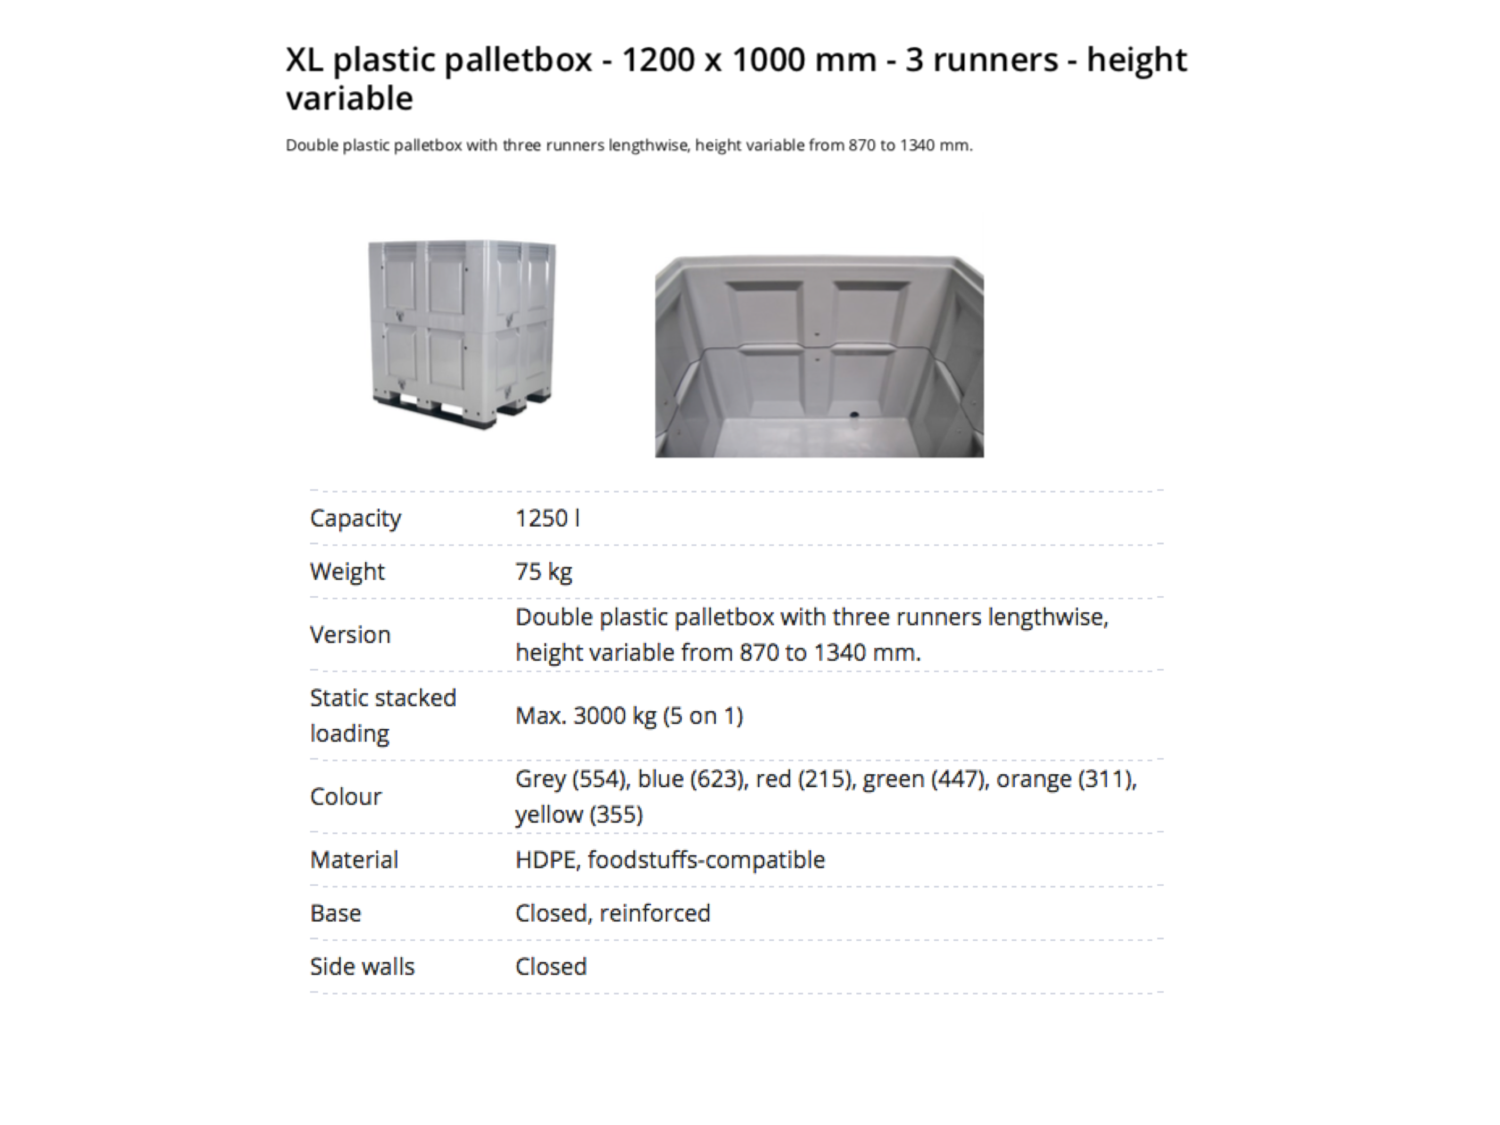
\includegraphics[width=0.5\textwidth]{dppd_11_2}
\end{dunefigure}

Following the \dword{ctsf} operations, the \dwords{pmt} are placed in a custom structure in \num{4} $\times$ \num{3} arrays. The structure is assembled with metal and plastic parts so the entire structure, together with the \dwords{pmt}, can be moved into the cleanroom underground. Three of these structures are placed on top of each other inside the boxes with the crane. The individual cartons that held the \dwords{pmt} get recycled at the \dword{ctsf}. The local movement of the transportation boxes in the \dword{ctsf} can be done with compact warehouse forklifts. The \dword{ctsf} will also be used as the storage area for the large \dword{pmt} transportation boxes before they are sent to \dword{surf}. The boxes are stored in single-shelf racks to the right and left of the entrance to the work area (Figure~\ref{fig:dppd_11_3}). The first set of boxes is placed on the floor and the second set on a shelf that is \SI{1.5}{\m} off the ground. This area can store the entire \dual \dword{pds} \dword{pmt} inventory of \dpnumpmtch \dwords{pmt} in \num{20} boxes. The \num{80} spare \dwords{pmt} can be placed in three boxes that can be stored on the floor in the available space in the work area as the \dual \dword{pds} \dword{ctsf} operations are finished.

The large \dword{pds} boxes, wrapped with plastic foil at the \dword{ctsf}, get opened in the material airlock underground. After removing the plastic wrapping, the transport boxes, with their entire contents, are moved into the cleanroom. A pallet jack can move the  \dword{pds} boxes around the underground areas. Each \num{4} $\times$ \num{3} structure is removed from the transportation box and moved inside the cleanroom by the crane. The structure goes into the dark box for functionality tests of the \num{12} \dwords{pmt}. The transportation boxes are used for storage before installation. Empty boxes are returned to \dword{ctsf}. At most, three \dword{pds} boxes are in the cleanroom at a time.

The \num{4} $\times$ \num{3} structure will be moved by crane into the cryostat and placed on the cryostat floor at a location convenient to the active installation area. The \dwords{pmt} will then be installed one by one. 

%\subsection{Integration and Testing Facility Operations}
\subsection{Coating, Testing and Storage Facility Operations}
\label{subsec:dp-pds-itf}

The \dword{ctsf}, of dimensions \SI{10}{\m} $\times$ \SI{8}{\m}, with a (\SI{12}{\ft}) ceiling equipped with a gantry crane, is the area planned for applying the \dword{tpb} coating on the \dword{pmt} windows, for \dword{qc} of the \dwords{pmt}, and for storage and preparation for transport to \dword{surf}. If the option of installing individual \dwords{gg} on the \dword{pmt} support structures, which is under consideration by the \dual \dword{pds} and \dword{hv} consortia, is %realized
implemented, this operation will also take place at the \dword{ctsf}. The layout of the \dword{ctsf} is shown in Figure~\ref{fig:dppd_11_3}.

\begin{dunefigure}[The layout of the \dshort{ctsf}]{fig:dppd_11_3}
{The layout of the \dword{ctsf}.}
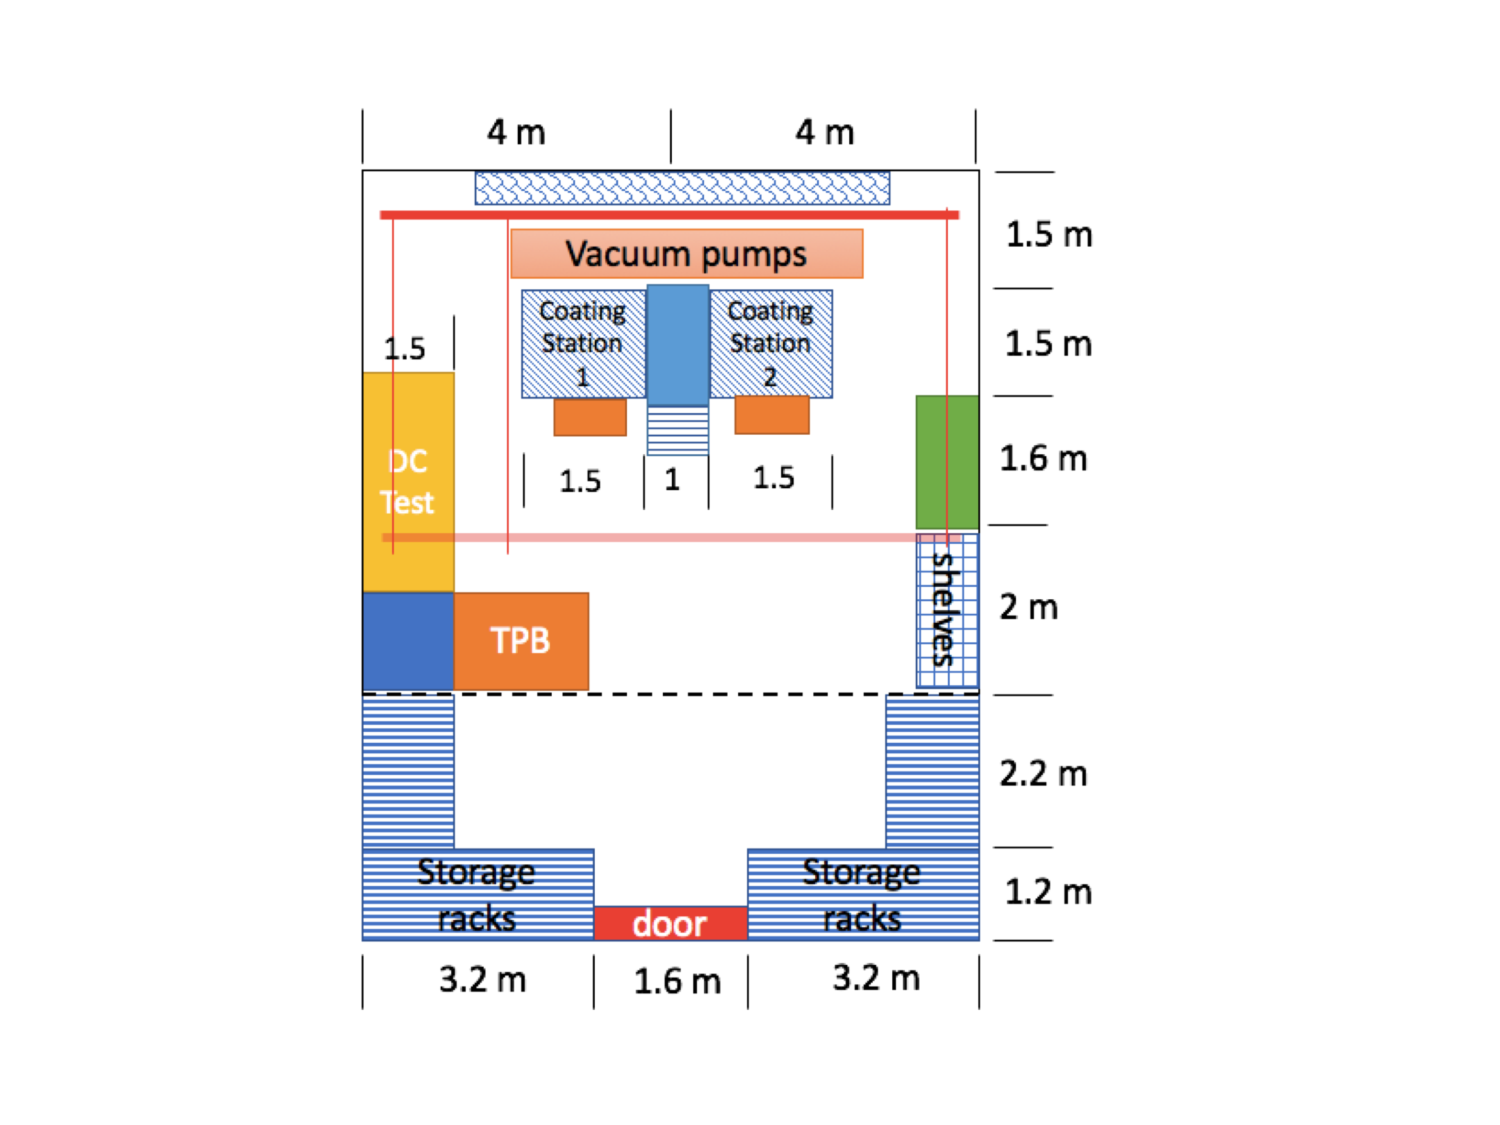
\includegraphics[width=0.4\textwidth]{dppd_11_3}
\end{dunefigure}

Two coating stations are planned with dimensions \SI{1.5}{\m} $\times$ \SI{1.5}{\m}. Figure ~\ref{fig:dppd_11_4} shows pictures of a \dword{tpb} coating station at the \dword{cern} thin-film facility. At \dword{surf}, an elevated platform, accessible by stairs, is placed between the two stations %. This platform will be used to reach 
to provide access to the top of the evaporator, which is approximately \SI{1.5}{\m} above ground level and inside the vessel. Cooling water, nitrogen, and electricity are provided from the outlets placed along the \SI{8}{\m} wall (indicated by wavy lines in Figure~\ref{fig:dppd_11_3}). Vacuum pumps are placed in the immediate vicinity of the evaporators. Control electronics are be placed next to the evaporator chambers. 

\begin{dunefigure}[Single \dshort{tpb} coating station]{fig:dppd_11_4}
{Pictures of a single \dword{tpb} coating station (courtesy of Wil Vollenberg, \dword{cern}-TE Department).}
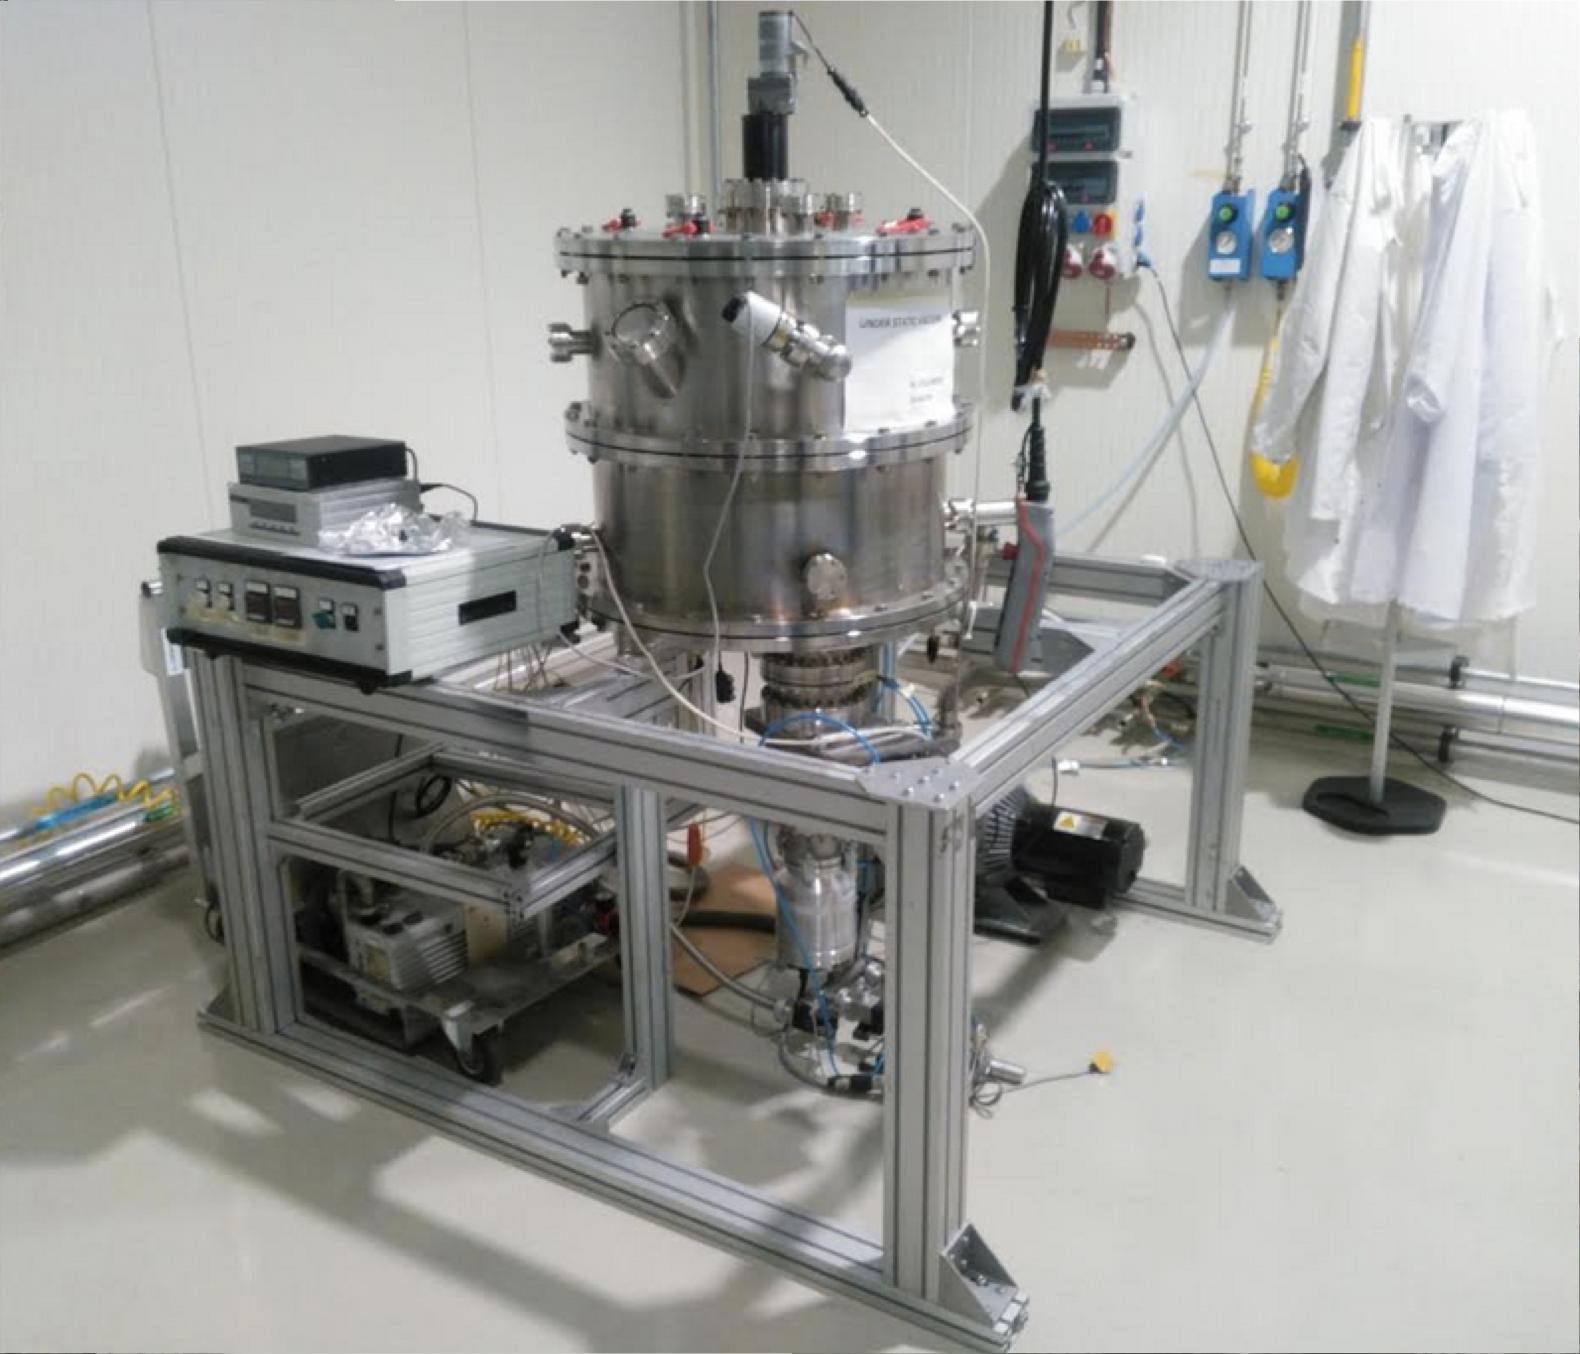
\includegraphics[height=8cm]{dppd_11_4_left.jpg}
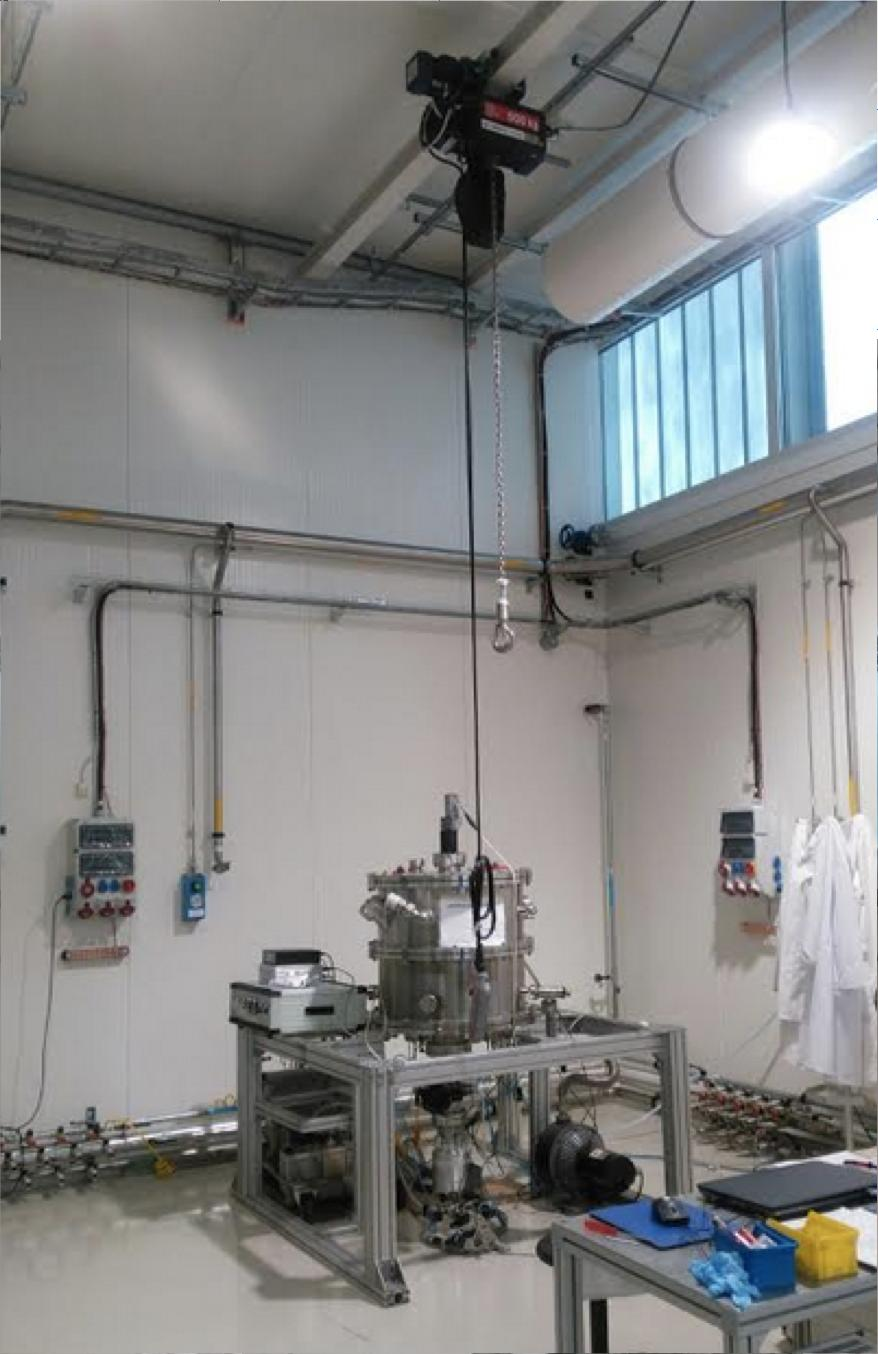
\includegraphics[height=8cm]{dppd_11_4_right.jpg}
%\includegraphics[height=8cm]{dppd_11_4} too big
\end{dunefigure}

%The \dwords{pmt} are removed from their individual cartons when they arrive at the \dword{ctsf}. While still in their cartons the \dwords{pmt} first undergo tests for basic functionality to verify that they have been safely transported from the remote sites. They will remain in these %boxes 
%cartons until the windows are coated. The \dword{pmt} windows will be cleaned with acetone and isopropanol before the evaporation. This will be done in the flow device/fume hood shown as a green box along the \SI{10}{\m} wall in Figure~\ref{fig:dppd_11_3}. The gantry crane (indicated with red bars in Figure~\ref{fig:dppd_11_3}) can move parts between the coating stations and the work desks, %. It will be used to 
%and remove the vessel lid and support it while the \dword{pmt} is installed for coating.
\fixme{check my edits in next pgraph. Order of operations was not clear. anne}
When they arrive at the \dword{ctsf}, and still in their cartons, the \dwords{pmt} first undergo tests for basic functionality to verify that they have been safely transported from the remote sites. They remain in these cartons while the windows are cleaned with acetone and isopropanol. The \dword{pmt} are then removed to be coated in the flow device/fume hood, shown as a green box along the \SI{10}{\m} wall in Figure~\ref{fig:dppd_11_3}. The gantry crane (indicated with red bars in Figure~\ref{fig:dppd_11_3}) moves parts between the coating stations and the work desks, %. It will be used to 
and removes the vessel lid and supports it while the \dword{pmt} is installed for coating.

Following the evaporation procedure, we install acrylic protective plates to cover the coated \dword{pmt} windows.
%, and the \dwords{pmt} will be placed in individual dark plastic protective bags. 
The \dwords{pmt} are tested again for basic functionality prior to attachment %. They will then be attached 
to the \num{4} $\times$ \num{3} structure in preparation for transportation to \dword{surf}.

At the \dword{ctsf}, the \dword{pmt} windows are coated at a rate of \num{4} \dwords{pmt}/day, i.e., \num{20} \dwords{pmt}/week and \num{80} \dwords{pmt}/month. Given the installation rate of \num{120} \dwords{pmt}/month, the \dword{ctsf} operations should start before installation begins. \dword{ctsf} has sufficient storage capacity for the entire \dword{pmt} inventory of the \dword{pds}. 

\subsection{Underground Installation and Integration}
\label{subsec:dp-pds-undergroundinstallation}

The cryostat cable/fiber installation precedes the installation of the \dword{fc}. The cables/fibers are routed from the flanges to the bottom of the cryostat. The total cable/fiber mass (length) is approximately \SI{50}{\kg} (\SI{25}{\m}) per sector, with an average mass/length of \SI{2}{\kg/\m}, where one sector comprises \num{36} \dwords{pmt} (see Section~\ref{sec:dp-pds-overview_layout}). The free ends of the cables/fibers are temporarily attached to the cryostat floor so that we can easily access them during installation. The cable/fiber and tray installation is done on both sides of the cryostat. At this stage, we transport the \dword{hv} cables %will be transported 
in a single box from the \dword{ctsf} to \dword{surf}. At the same time, we transport a separate box containing \num{120} calibration fiber plus fiber bundle assemblies %will be transported 
 from the \dword{ctsf} to %\surf. The boxes %will be transported 
 to the cryostat roof in order to hang the cables/fibers %can be hung 
 through the feedthroughs for installation in the cable trays.  

Once the plastic wrap is removed, the \dword{pds} \dword{pmt} box and its entire contents can be moved to the cleanroom. The \dwords{pmt} undergo functionality tests inside the custom design dark box, which can cover the entire structure of \num{4} $\times$ \num{3} \dwords{pmt}. The dark box will have a \dword{hv} patch panel and allow consecutive tests of all \num{12} \dwords{pmt} in one testing session without intervention. The test is a simple check for healthy \dword{pmt} operations. Once the operation of the \dwords{pmt} is verified, the structure can be moved into the cryostat.

Inside the cryostat, the \dwords{pmt} is removed from the structure. %The window protections will be kept on the \dwords{pmt}. 
The \dwords{pmt} are mounted on the membrane floor in the areas between the membrane corrugations using their support structures. The attachment is done using a stainless steel support base that can be point-glued to the membrane. The weight of the support and the \dword{pmt} exceeds the buoyancy force of the system. Furthermore, these supports %also 
ensure stability against possible lateral forces acting on the \dwords{pmt} due to the liquid flow. Once the attachment is complete, we connect the short \dword{hv} cables to the cold \dword{hv} cables with SHV barrel connectors, and route the calibration fibers  to the support structure  and connect them. Once all the \dwords{pmt} of a given \dword{pds} sector are installed, the cables and fibers will be fixed in their final positions.

The installation rate is planned at \num{30} \dwords{pmt}/week. After installation, we return the empty \dword{pmt} boxes and the transport structures to \dword{ctsf}.

Table~\ref{tab:dppd_t_11_1} summarizes the quantities related to the \dual \dword{pds} installation.

\begin{dunetable}
[Quantities related to the \dual \dshort{pds} installation.]
{lc p{0.8\textwidth}}
{tab:dppd_t_11_1}
{Quantities related to the \dual \dword{pds} installation.}
Parameter & Value \\ \colhline
Number of \dual \dshort{pds} sectors	& \num{20} \\ \colhline
Number of \dshorts{pmt} per sector	& \num{36} \\ \colhline
Number of calibration fibers per sector	& \num{6} \\ \colhline
Number of feedthrough flanges per sector	& \num{1} \\ \colhline
Total number of feedthrough flanges	& \num{20} \\ \colhline
Number of \dshort{hv} racks per sector	& \num{1} \\ \colhline
Frequency of transportations to \surf from \dshort{ctsf}	& \num{4} PDS boxes/month \\ \colhline
Rate of installation	& \num{30} PMTs/week \\
\end{dunetable}

The reflector/\dword{wls} panels are assembled into a unit panel assembly on a dedicated table underground immediately prior to the installation, following the procedure described in Section~\ref{sec:dp-pds-mechanics}. They are placed in a storage structure that can hold three regular and two extended reflector/\dword{wls} panel assemblies, which get installed in one row of an \dword{fc} super-module. The installation of the panel assemblies will be synchronized with the installation of the \dword{fc} modules, described in Section \ref{sec:fddp-hv-transport-install} and depicted in Figure~\ref{fig:dp-super-module-installation-secuence}. Once a row of the \dword{fc} super-module is installed, we mount the five reflector/\dword{wls} panel assemblies  on the \dword{frp} I-beams of the \dword{fc} submodules, starting from one end of the row and progressing towards the other. Figure \ref{fig:dppd_reflective_panel_installation_sequence} depicts the installation sequence of a unit reflector/\dword{wls} panel. The sequence is as follows: %can be described as below:

\begin{enumerate}
\item Put the top two screws accessing the back side through the top liquid-flow opening (Figure~ \ref{fig:dppd_reflective_panel_installation_sequence}  left).
\item Place two nuts in the closed holes of the long holding bar. Slide the long bar behind the panel to the level of the middle bar by holding it through the central liquid-flow opening. Put the two middle bar screws and remove the long bar through the bottom liquid-flow opening after sliding it all the way down (Figure~ \ref{fig:dppd_reflective_panel_installation_sequence} center).
\item Put the bottom two screws accessing the back side through the bottom liquid-flow opening (Figure~ \ref{fig:dppd_reflective_panel_installation_sequence}  right).
\end{enumerate}

\begin{dunefigure}[Installation sequence of unit reflector/\dshort{wls} assembly on  \dshort{fc} I-beams]{fig:dppd_reflective_panel_installation_sequence}
{The schematic view of the installation sequence of a unit reflector/\dword{wls} panel assembly on the \dword{fc} I-beams: The installation of the top two screws (left), the middle two screws with the holding bar (center) and the bottom two screws (right). The I-beams are shown as blue vertical rectangles at each side of the panel assembly, the panels as grey squares, and the horizontal support bars and the holding bar as green rectangles. The screw locations are indicated with thin red arrows.}
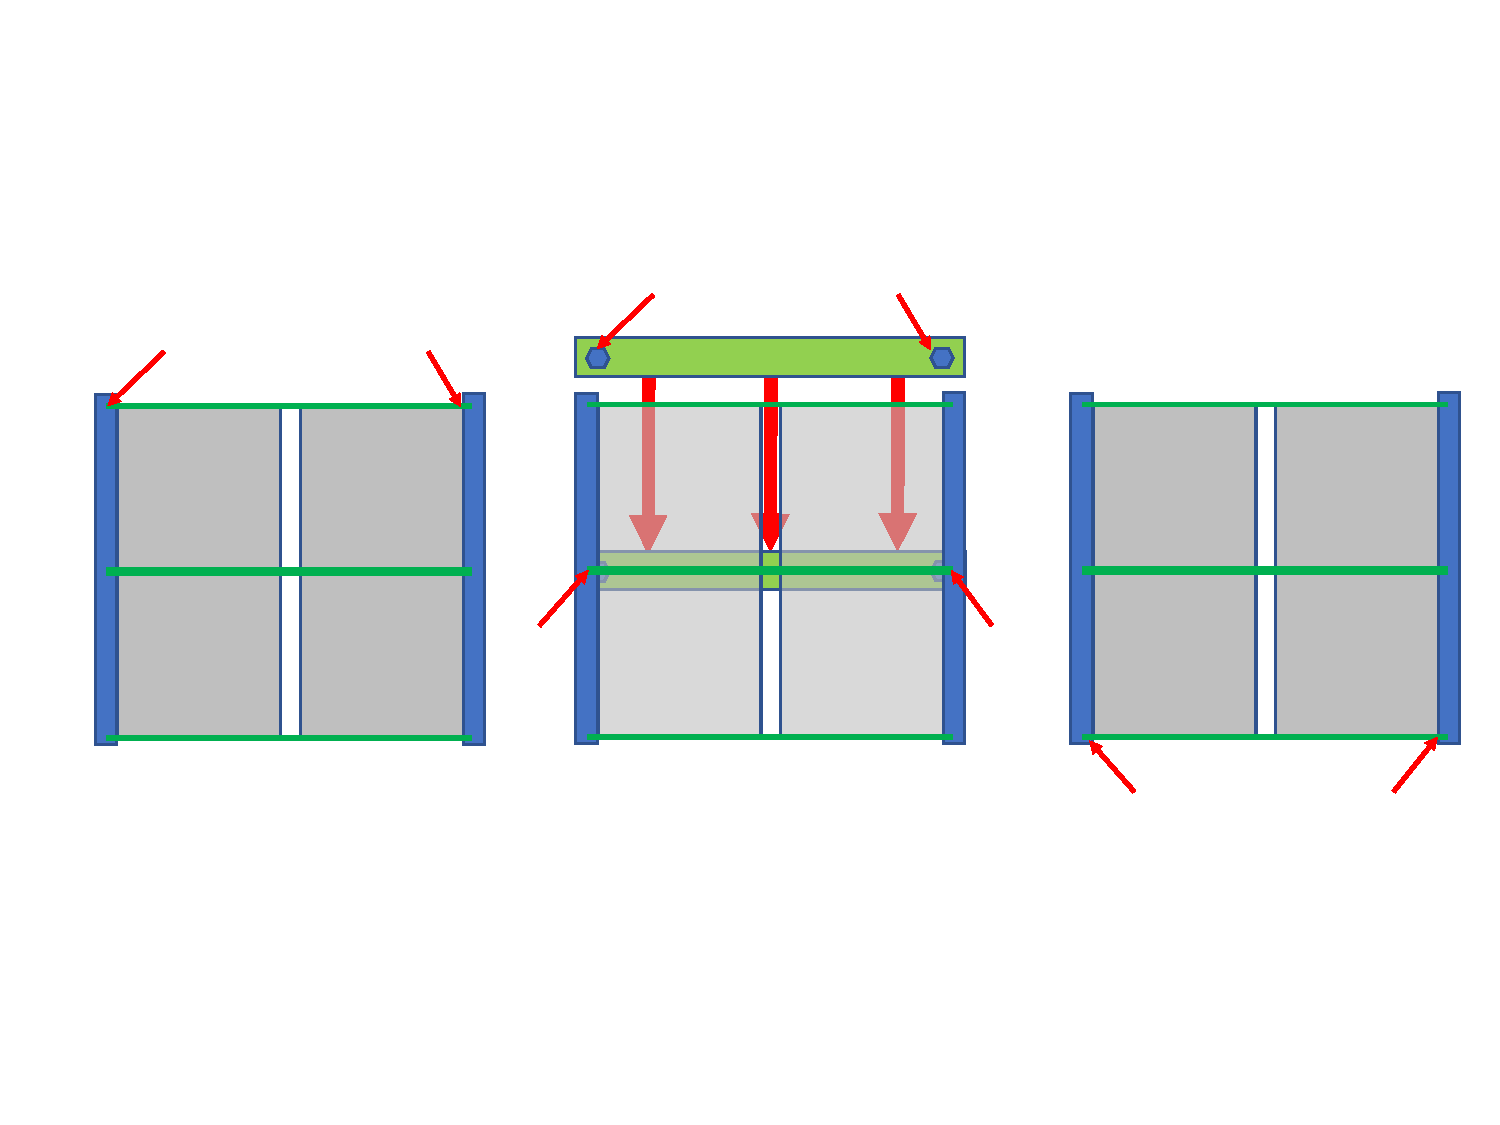
\includegraphics[width=0.8\textwidth]{dppd_reflective_panel_installation_sequence}
\end{dunefigure}

\subsection{Commissioning}
\label{subsec:dp-pds-commissioning}

The commissioning of the \dword{pds} is performed in partitions. The \dword{daq} and the \dword{hv} systems will determine, in large part, the size of a single partition, and the \dword{daq} and \dword{hv} partitions, along with the relevant control systems,  are commissioned before connecting the \dwords{pmt} to these systems.

%The exact availability of the cryostat as a sufficiently dark environment depends on the overall installation schedule. Once it is possible, the \dwords{pmt} are powered up, and basic functionality and performance checks are carried out. These include pedestal data taking, i.e., recording event data with external periodic triggering, and tests with the calibration system where the data taking is triggered in synchronization with a light source, as described in Section \ref{sec:dp-pds-calibration}.
The point at which the cryostat becomes available as a sufficiently dark environment depends on the overall installation schedule. At that point, the \dwords{pmt} are powered up, and basic functionality and performance checks are carried out. These include pedestal data taking, i.e., recording event data with external periodic triggering, and tests with the calibration system where the data taking is triggered in synchronization with a light source, as described in Section~\ref{sec:dp-pds-calibration}.

The commissioning tests will validate the basic performance characteristics of the \dwords{pmt}, e.g., the dark count rate and gain, and allow identifcation and elimination of %issues 
any problems related to installation. % can then be identified and eliminated. 
A commissioned sector becomes a part of the overall detector and can join the global calibration data taking and commissioning.


